
\documentclass{article}

\usepackage{geometry}
\usepackage{amsmath}
\usepackage{soul}
\usepackage{color}
\usepackage{amssymb}
\usepackage{graphicx}
\usepackage{float}
\usepackage{cancel}
\usepackage{setspace}
\usepackage{listings}
\usepackage{hyperref}

%\definecolor{lightgrey}{rgba}{.824, .825, .825}
\definecolor{lightgrey}{rgb}{.867, .894, .886}

% no indentation
\setlength{\parindent}{0cm}

\lstdefinestyle{code}{
    backgroundcolor=\color{lightgrey},
    breaklines=true,
    numbers=left,
	basicstyle=\small,
    tabsize=4,
    language=Python
}
\lstset{style=code}

\newcommand{\mathsym}[1]{{}}
\newcommand{\unicode}[1]{{}}
\newcommand{\pd}[2]{\frac{\partial #1}{\partial #2}}

\newcommand{\eig}{\text{eig}}
\newcommand{\abs}{\text{abs}}

%\geometry{a4paper, left=2cm, right=2cm, top=1cm, bottom=2cm}
\geometry{a4paper, bottom=4cm}

\title{ME 793 Project \# 2}
\author{Brooks Karlik}
\date{\today}

\newcommand{\rank}{\text{rank}}
%\setlength{\parindent}{0.0pt}


\begin{document}

\maketitle
\newpage

\section{Introduction}

In this paper, we present solutions to the Sod Shock Tube problem, originally proposed by Gary
Sod in 1978. The problem involves solving the one dimensional Euler equations with a sharp
discontinuity in pressure and density at the midsection of a 10m tube. 
Solutions are generated using the Lax Friedrichs scheme, Lax Wendroff 2 step 
scheme, and the Lax Wendroff scheme with artificial viscosity. Full code is available 
at \url{https://github.com/vanillaBrooks/finite-volume}

\section{Methods}

The one dimensional Euler equations are specified by equations \ref{eq_euler} and \ref{eq_qf}.

\begin{equation}
	\frac{
		\partial \boldsymbol{q}
	}{
		\partial t
	}
	+
	\frac{
		\partial \boldsymbol{F}
	}{
		\partial t
	}
	=
	0
	\label{eq_euler}
\end{equation}
\begin{equation}
	\boldsymbol{q}
	=
	\begin{bmatrix}
		\rho \\
		\rho u \\
		\rho \left(e + \frac{1}{2} u^2\right)
	\end{bmatrix}
	\quad
	\boldsymbol{F}
	=
	\begin{bmatrix}
		\rho u \\
		\rho u^2 + p \\
		u 
		\left(
			p + \rho
			\left(
				e + \frac{1}{2} u^2
			\right)
		\right)
	\end{bmatrix}
	\label{eq_qf}
\end{equation}

The Lax-Friedrichs (LF) scheme is give by equation \ref{eq_LF}. A grid resolution study was performed using
the LF scheme and is plotted in figure \ref{fig_n_compare}. A higher number of grid points results
in more refined peaks in the plots.
Using the results of the grid resolution study, a 
final value of $n=1501$ was used for plotting purposes in combination with a conservative CFL number of 0.1.

\begin{equation}
	q_{j}^{n+1}
	=
	\frac{1}{2}
	\left(
		q_{j+1}^n
		+
		q_{j-1}^n
	\right)
	-
	\frac{\Delta t}{2h}
	\left(
		F_{j+1}^n
		-
		F_{j-1}^n
	\right)
	\label{eq_LF}
\end{equation}


\begin{figure}[H]
	\centering
	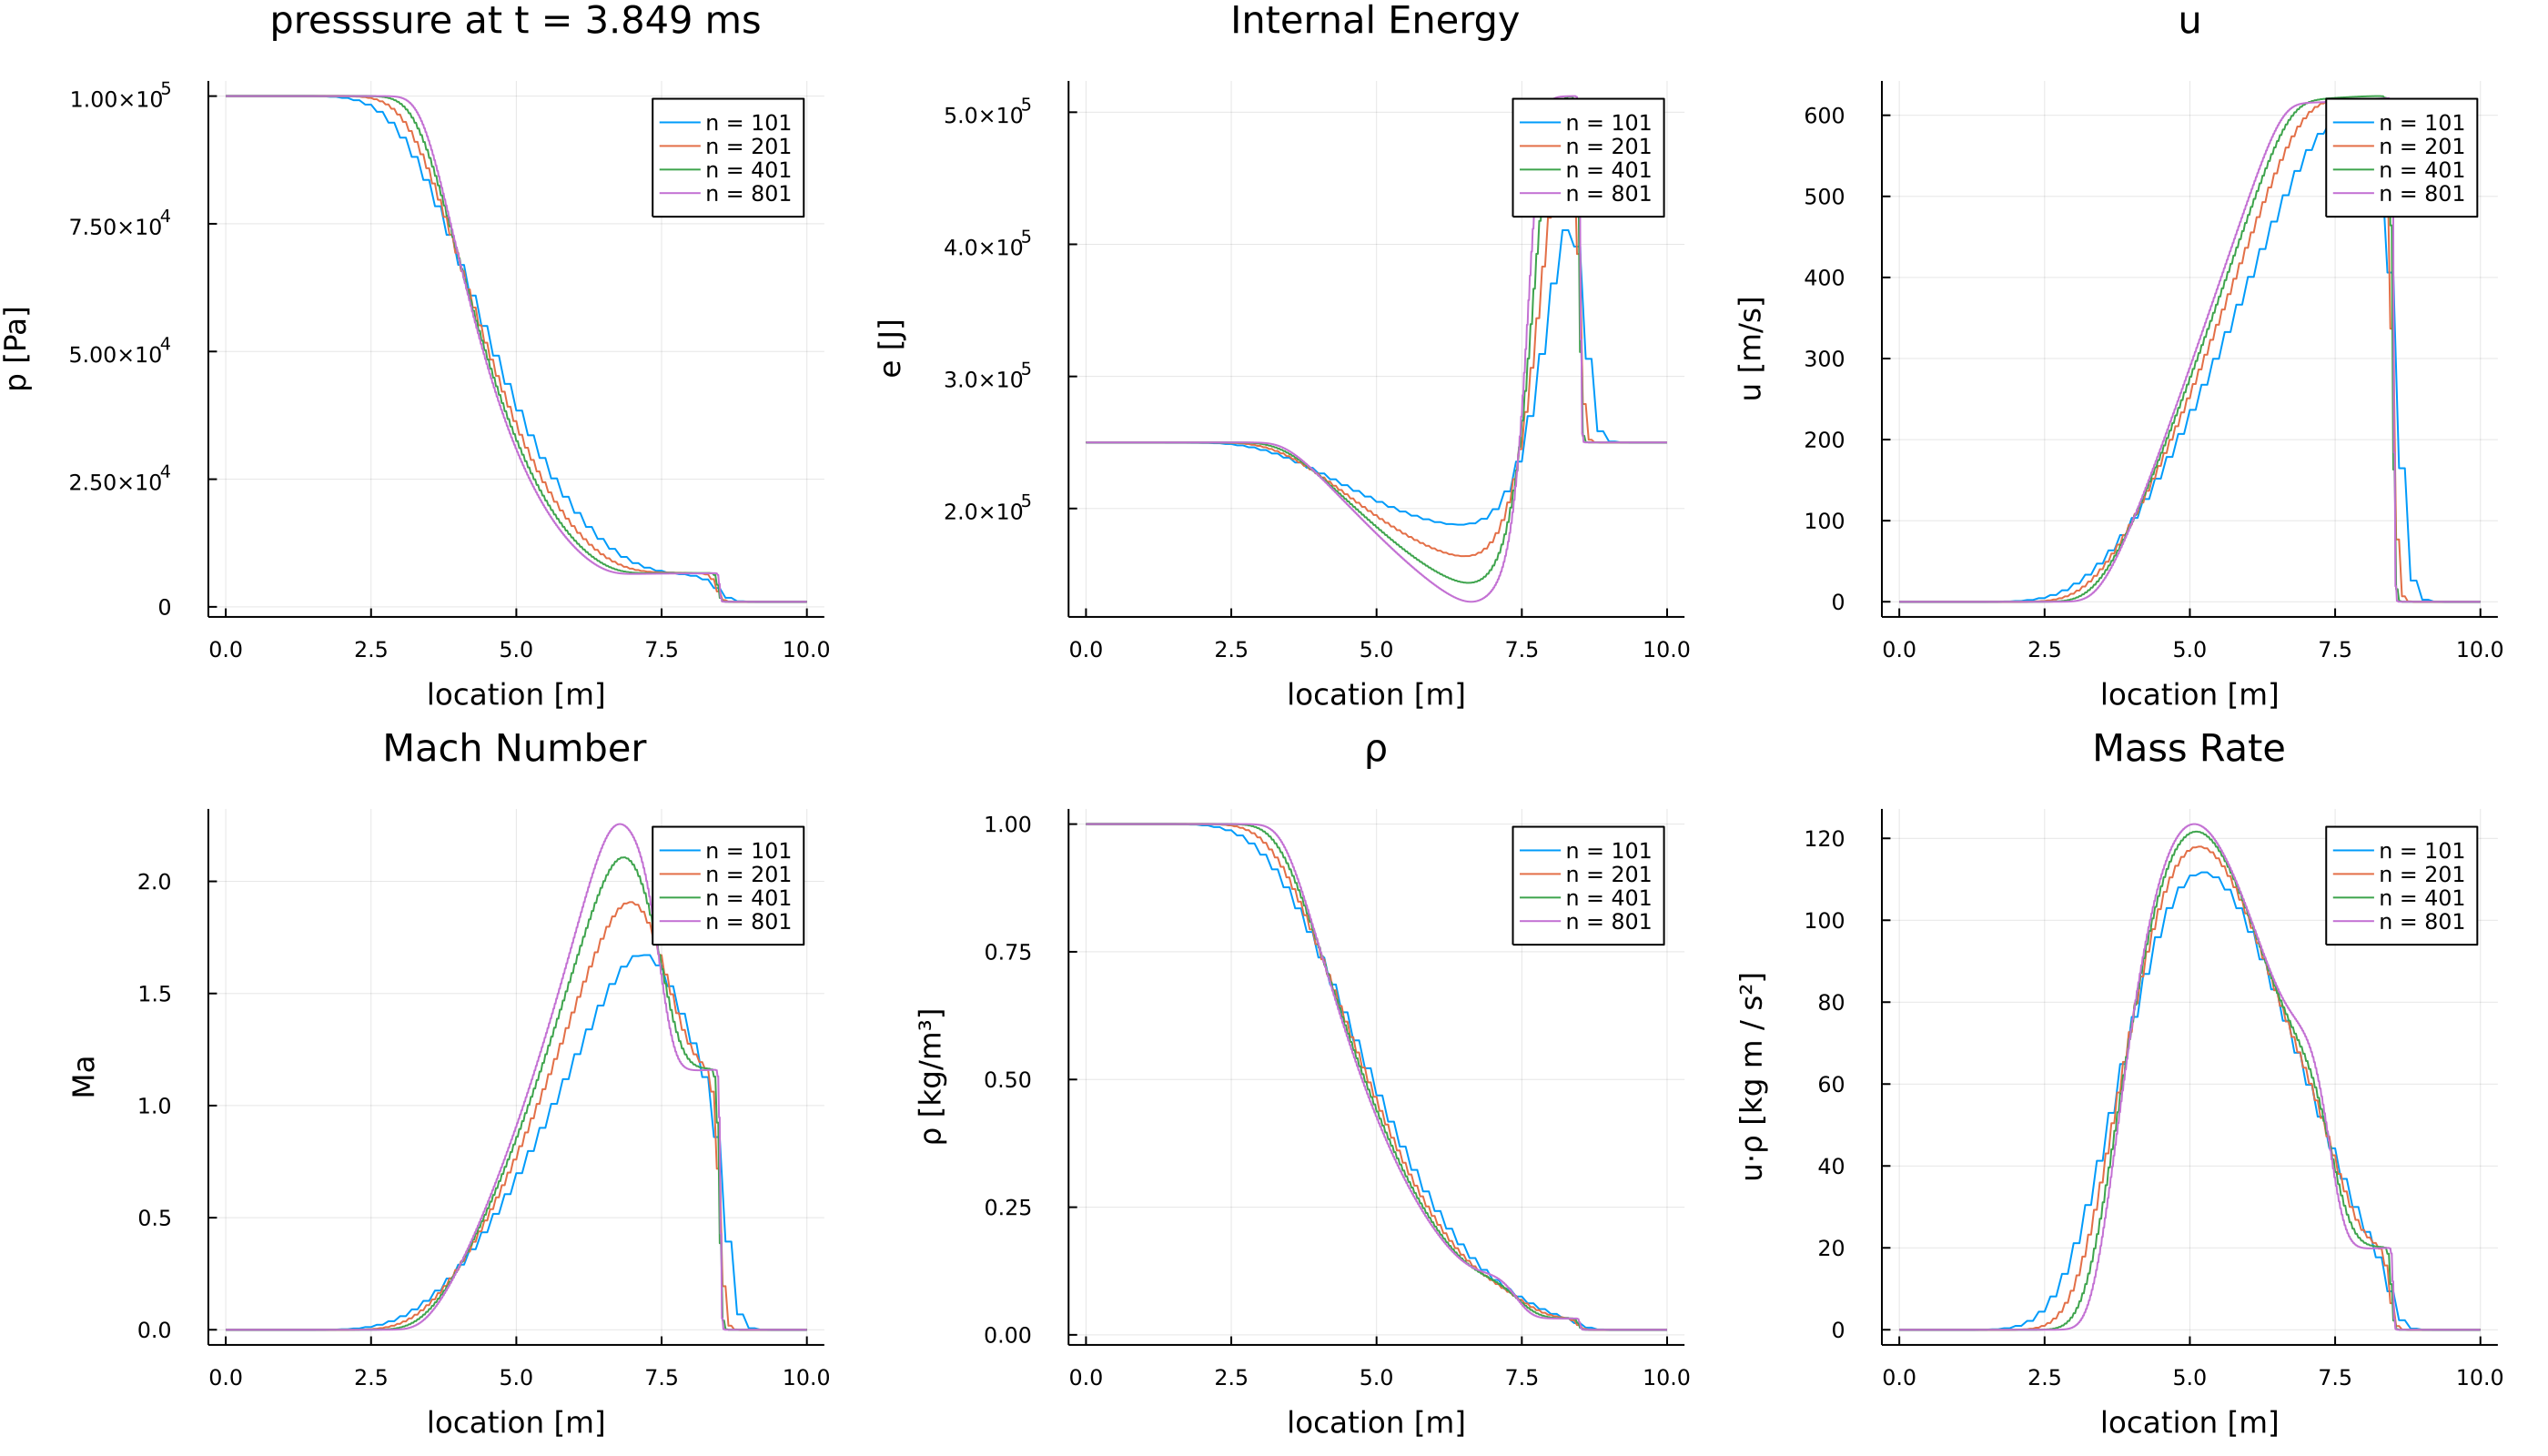
\includegraphics[width=\textwidth]{./figs/n_compare.png}
	\label{fig_n_compare}
	\caption{A grid resolution study performed using the LF method}
\end{figure}

The Lax-Wendroff 2-step scheme (LW-II) is given by equations \ref{eq_LW_1} and \ref{eq_LW_2}. Since the 
LW-II scheme is subject to oscillations resembling Gibbs phenomena, an artificial flux may be added to the 
half step $F$ using equation \ref{eq_flux_adjustment}.

\begin{equation}
	q_{j+1/2}^*
	=
	\frac{1}{2}
	\left(
		q_{j}^{n}
		+
		q_{j+1}^n
	\right)
	+
	\frac{\Delta t}{2h}
	\left(
		F_{j+1}^n
		+
		F_{j}^n
	\right)
	\label{eq_LW_1}
\end{equation}

\begin{equation}
	q_{j}^{n+1}
	=
	q_j^{n}
	+
	\frac{\Delta t}{2}
	\left(
		F_{j+1/2}^*
		-
		F_{j-1/2}^*
	\right)
	\label{eq_LW_2}
\end{equation}

\begin{equation}
	F^*
	= 
	F^* 
	- 
	\alpha h^2 \rho
	\text{ }
	\abs
	\left(
		%du/du
		\pd{u}{x}
	\right)
	\pd{u}{x}
	\begin{bmatrix}
		0 \\
		1 \\
		u
	\end{bmatrix}
	\label{eq_flux_adjustment}
\end{equation}

\section{Results}

Figure \ref{fig_method_compare} provides an overview of the solutions plotted against each other. While the LF scheme
provides a good overview of the shape of the solution, the LW-II schemes better capture the sharp discontinuities
in the solution. The tradeoff in the LW-II schemes is the introductions of oscillations near discontinuities. Artificial
viscosity introduction (a la equatin \ref{eq_flux_adjustment}) does not show a significant improvement in the
shape of the solutions as compared to the regular LW-II schemes ($\alpha = 0$).\\

A comparison of different $\alpha$ values in the flux adjustment is located in figure \ref{fig_alpha_compare}. Large
differences in $\alpha$ values fail to produce significant changes in the solution.

\begin{figure}[H]
	\centering
	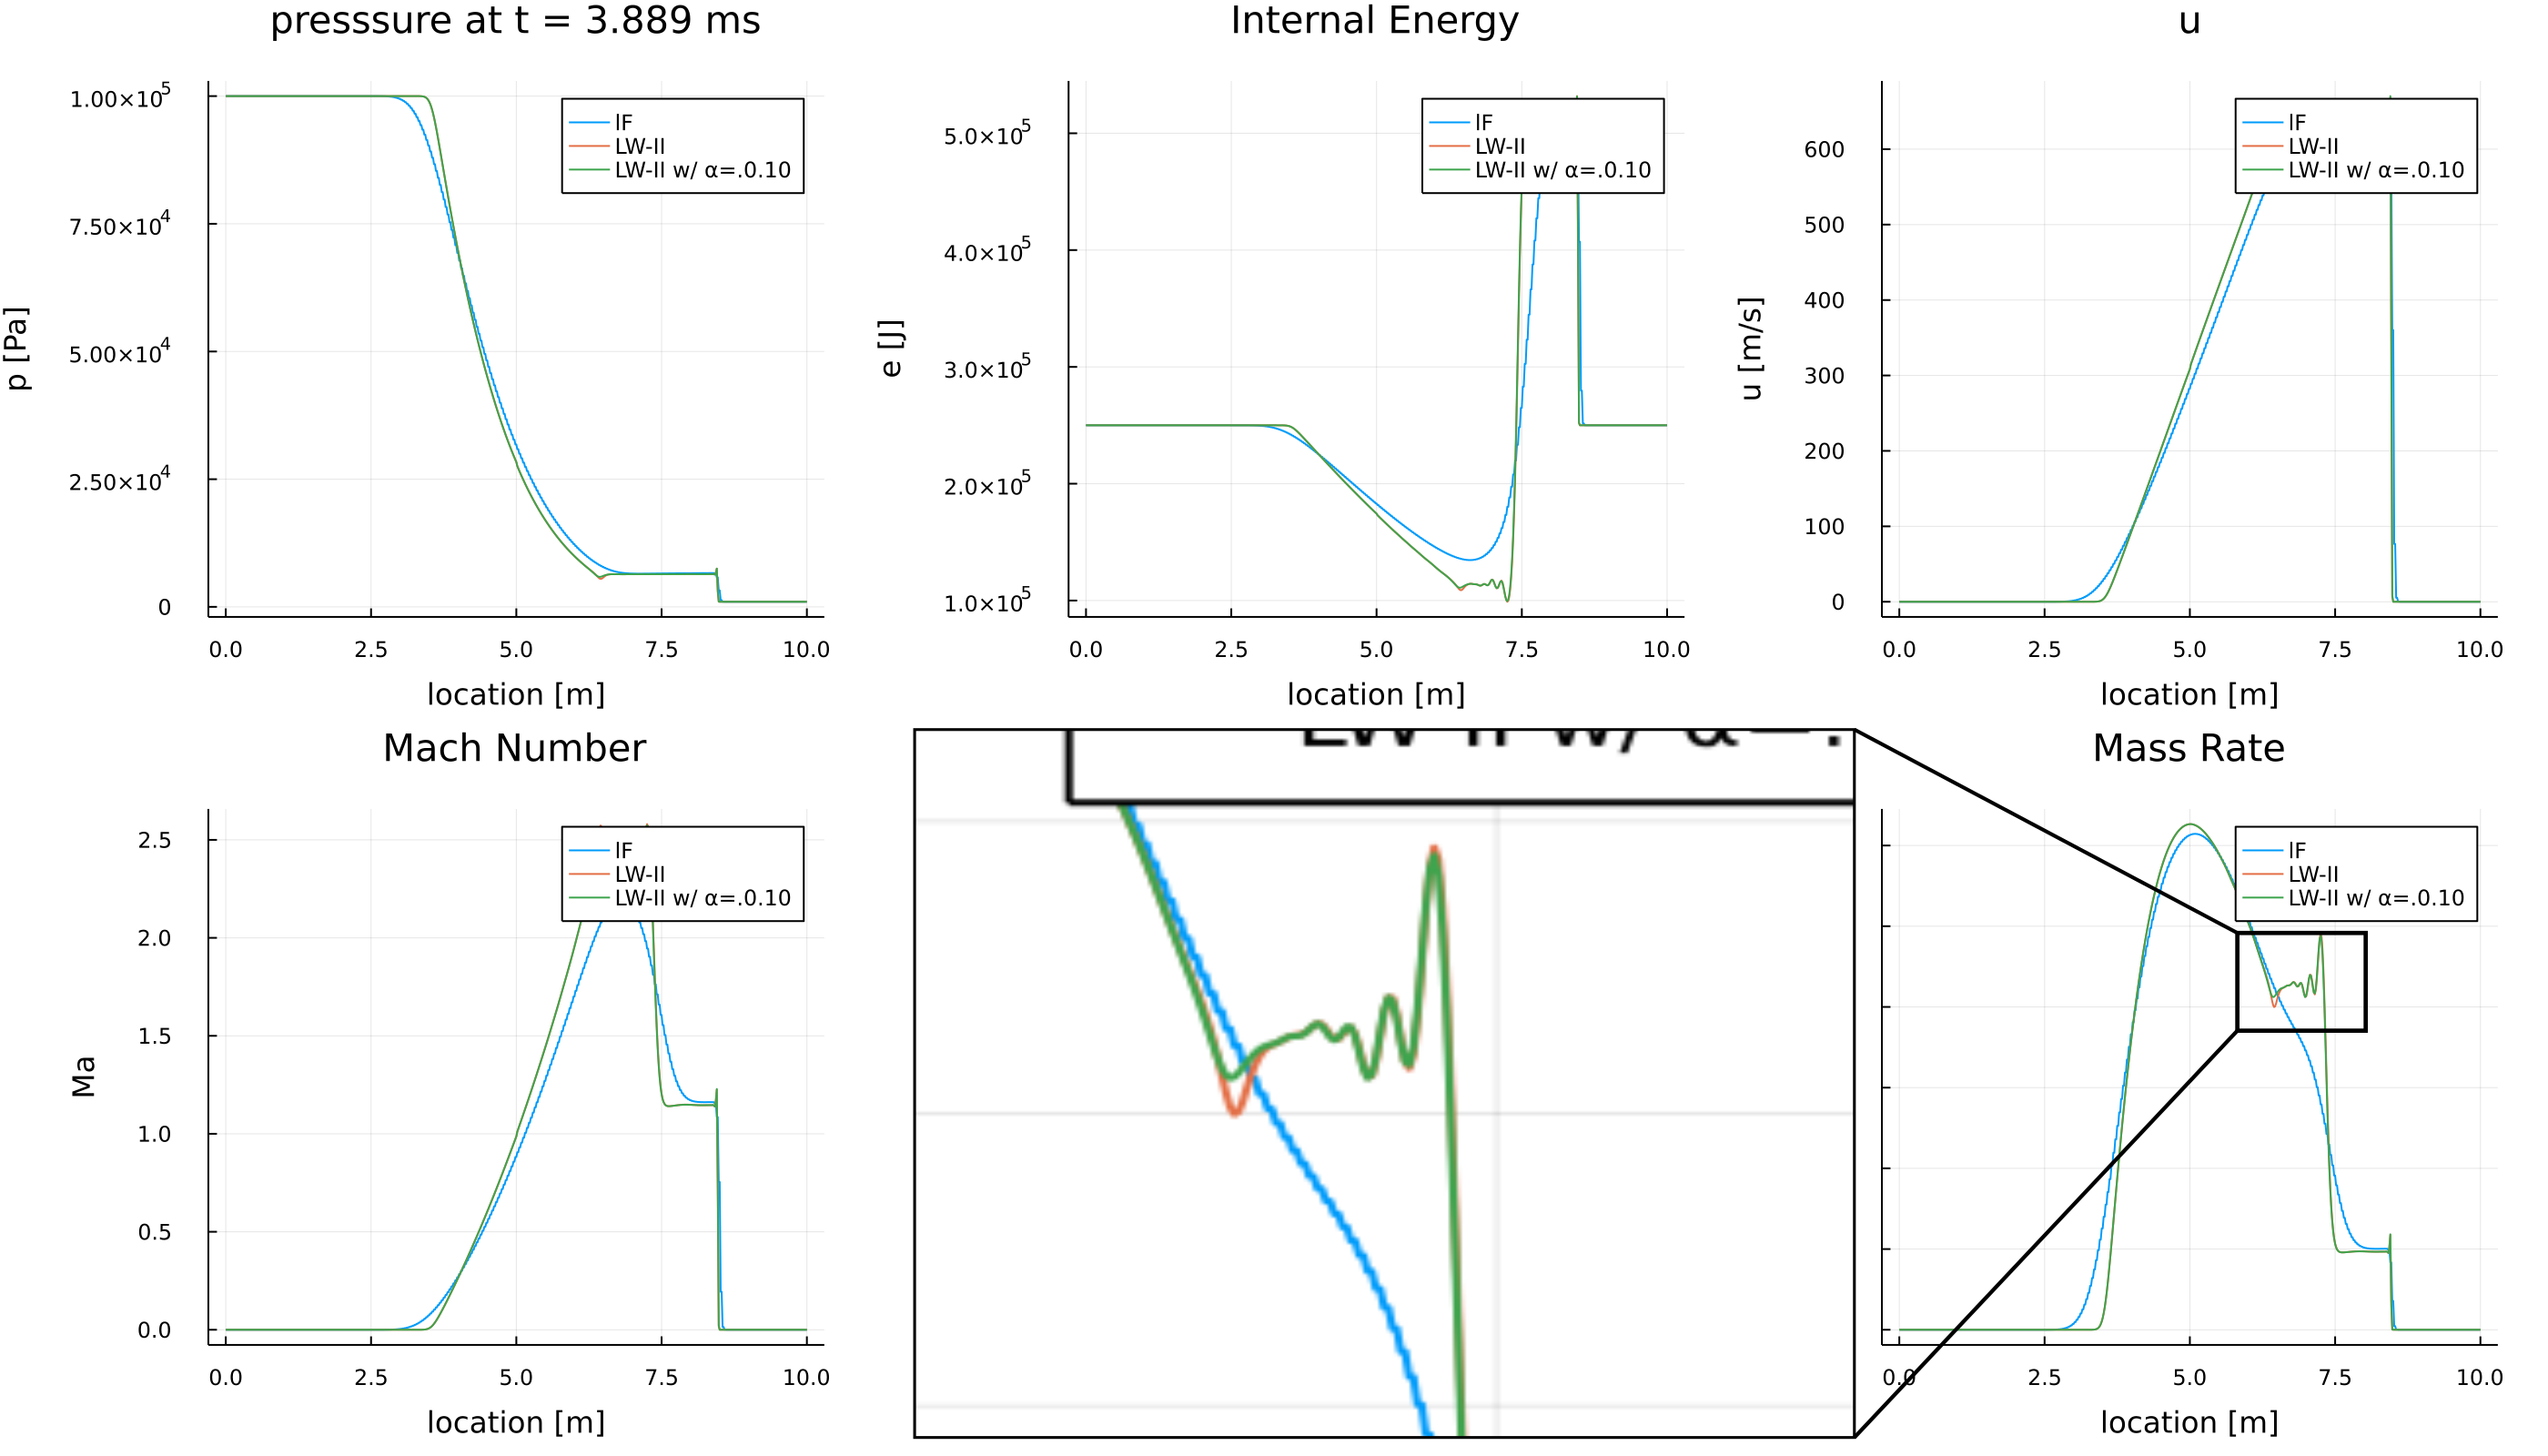
\includegraphics[width=\textwidth]{./figs/method_compare_nice.png}
	\label{fig_method_compare}
	\caption{A qualitative comparison of the three methods. The artificial flux added to the LW-II scheme
		does not produce significant changes in the solution.
	}
\end{figure}

\begin{figure}[H]
	\centering
	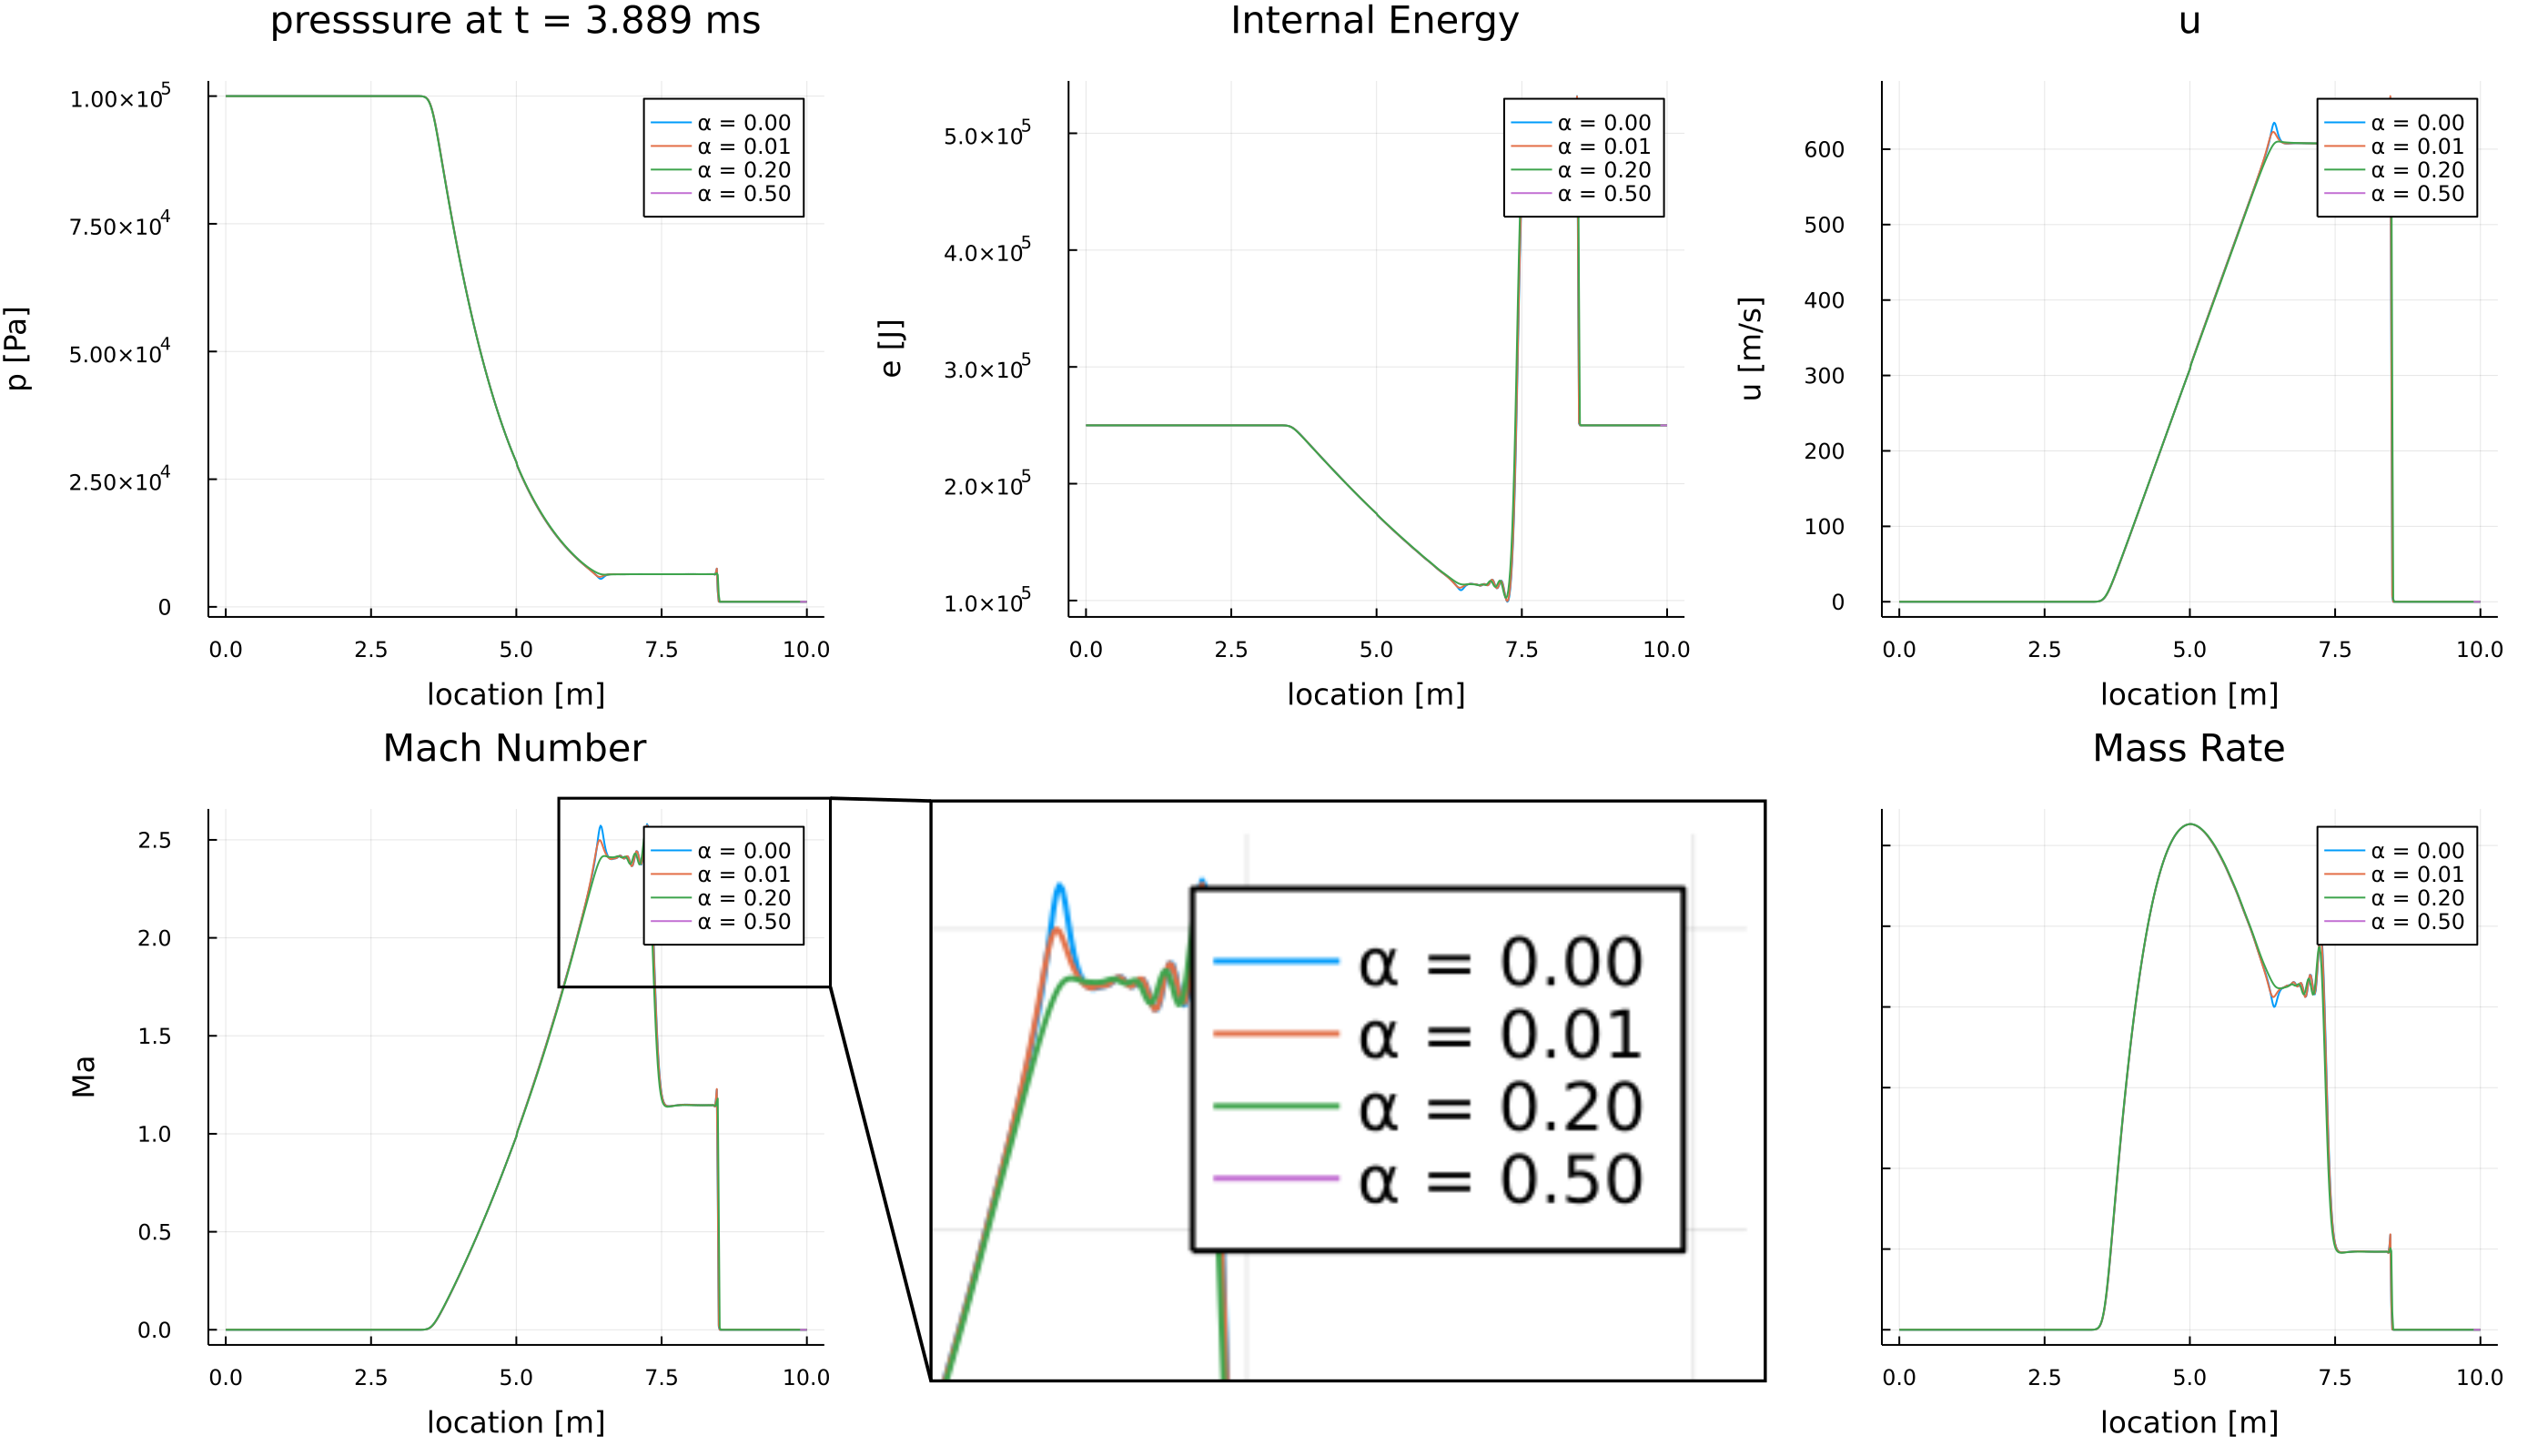
\includegraphics[width=\textwidth]{./figs/alpha_compare_nice.png}
	\label{fig_alpha_compare}
	\caption{A comparison of the $\alpha$ value used in artificial flux construction on the shape of the solution.
		The choice of $\alpha$ value does not produce significant differences in the solution.
	}
\end{figure}

\end{document}
